\section{增量式优化方法}

以\citeauthor{kaess2008isam}提出的iSAM系列文章为例(iSAM\citep{kaess2008isam}和iSAM2\citep{kaess2012isam2}),增量式集束优化算法很好地利用了SLAM集束优化问题的稀疏性和局部性,实现了高效的求解。iSAM系列的文章提出:
\begin{itemize}
    \item 对观测的雅各比矩阵(measurement Jacobian matrices)或者信息矩阵(information matrix)进行分解得到平方根信息矩阵(square root information matrix)的过程,等同于对因子图转化成贝叶斯置信网络的过程;
    \item 矩阵分解时产生的填充现象(fill-in),则等同于因子图转化过程中,多出来的变量之间的边;
    \item 同样,在矩阵分解时,选定不同的主元顺序(pivoting)对应于因子图转化过程中变量的消去顺序,其所产生的填充现象的程度也是不同的(见图\ref{fig:fill_in})。
\end{itemize}

因此,完全可以用分析因子图的转化过程来代替对矩阵分解过程的分析。具体来说,iSAM系列算法通过一种特殊的贝叶斯树的结构编码了平方根信息矩阵的结构,使得每次更新平方根信息矩阵时只要做很少的改动即可:
\begin{enumerate}
    \item \textbf{减少填充现象:}通过一些启发式算法如COLAMD\citep{davis2004algorithm}、CHOLMOD\citep{chen2008algorithm}算法找到次优(suboptimal)的变量消去顺序,使得因子图转化为贝叶斯置信网络的过程中尽可能地不产生新的边;
    \item \textbf{使用贝叶斯树编码平方根信息矩阵:}对于因子图转化而来的贝叶斯置信网络,使用特殊的贝叶斯树来编码其中的稀疏结构和变量因果关系;
    \item \textbf{即时重新线性化:}利用贝叶斯树中的编码的变量因果关系,每当因子图中加入新的变量或约束,则即时地对影响到的变量进行线性化,避免每次都重新构造整个平方根信息矩阵;
    \item \textbf{局部变量更新策略:}通过设置一个阈值$\epsilon$,在求解得到变量的增量$\Delta$后,根据其是否满足$|\Delta|>\epsilon$来判断是否需要更新这个变量。
\end{enumerate}

\begin{figure}[htb]
    \centering
    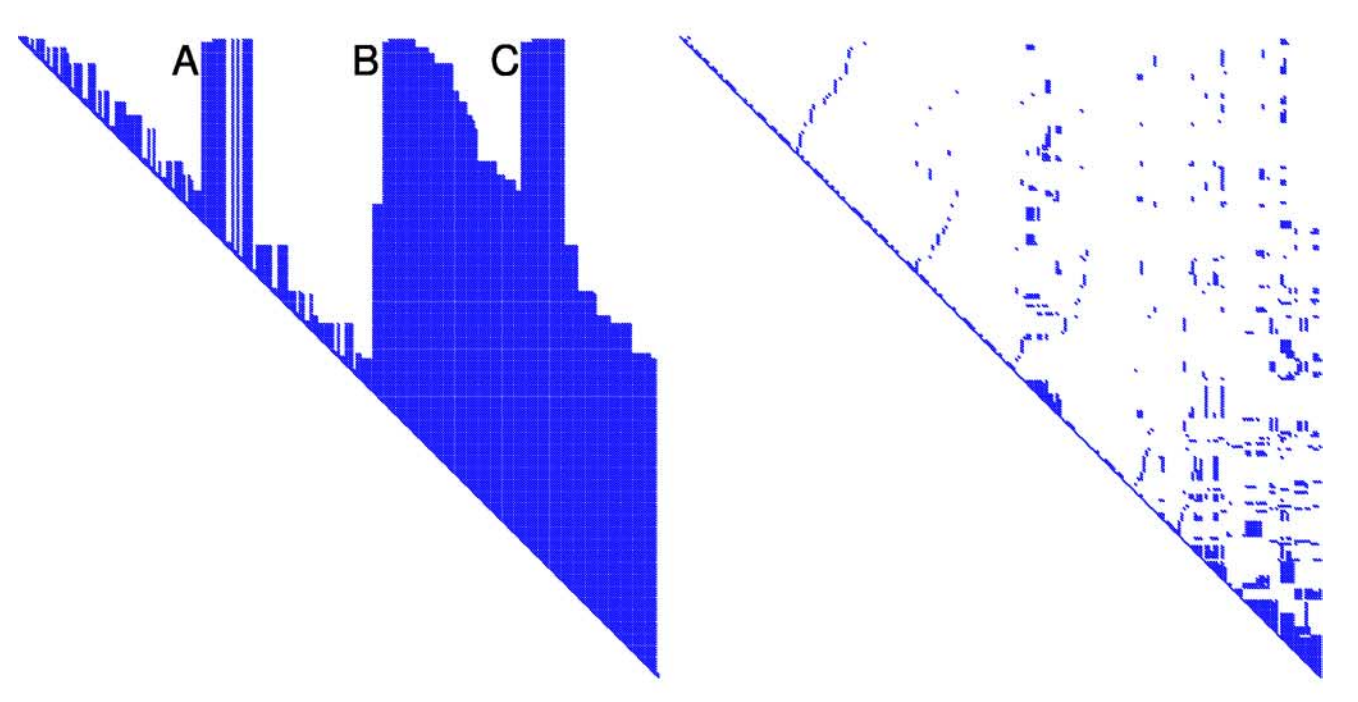
\includegraphics[width=.8\textwidth]{./figs/sparse_pattern.png}
    \caption{信息矩阵稀疏结构\citep{kaess2008isam}:左图代表按照一般的消元顺序得到的平方根信息矩阵,右图代表先使用COLAMD算法选择一个较优的消元顺序,然后得到的平方根信息矩阵。可见,变量消去顺序对矩阵分解产生的填充现象有巨大影响。}
    \label{fig:fill_in}
\end{figure}
